\documentclass{beamer}
\usetheme{Berlin}

\usepackage{graphicx}
\usepackage{grffile}
\usepackage{wrapfig}
\usepackage[ngerman]{babel}
\usepackage[utf8x]{inputenc}
\usepackage{hyperref}
\usepackage{subfigure}

\usepackage{todonotes}
\presetkeys{todonotes}{inline}{}
\let\todox\todo
\renewcommand\todo[1]{\vspace{0.3em}\todox[inline, size=\small , color=red!20]{#1}}

\begin{document}

\title{Performanz-Evaluation von Graphdatenbanksystemen versus MySQL am Beispiel von Kookkurrenzgraphen}
\author{Martin Junghanns, Sascha Ludwig \& Robert Schulze\\(IR\_{}15)} 
\date{\today}
\logo{
\includegraphics[scale=0.14]{uni_leipzig_logo}}
\setbeamertemplate{navigation symbols}{}

\begin{frame}
	\titlepage
\end{frame}

\begin{frame}\frametitle{Inhalt}
	\tableofcontents
\end{frame}

\section{Einleitung}

\begin{frame}\frametitle{Aufgabenstellung}
	\begin{itemize}
		\item Kennenlernen der Konzepte verschiedener Graphdatenbanken
		\item Implementierung eines Java-Frameworks zur Durchführung von Benchmarks
		\item Gegenüberstellung mit einer relationalen Datenbank (MySQL)
		\item Wortschatz Leipzig Projekt als Datenbasis
		\item Visualisierung und Auswertung der Messergebnisse
		\item Empfehlung zu Graphdatenbanken
	\end{itemize} 
\end{frame}

\begin{frame}\frametitle{Graphdatenbanken --- Allgemein}
	\begin{itemize}
		\item Verwaltung stark vernetzter Daten
		\item (explizite) Datenmodellierung als Graph		
		\item Performanz durch Vermeidung von Verbundoperation
		\item Schemafreiheit
		\item Anwendungen: Soziale Netzwerke, Recommendation, Transportnetze, Komplexe Softwaremodelle
	\end{itemize} 
\end{frame}

\begin{frame}\frametitle{Graphdatenbanken --- Auswahl für den Vergleich}
	\begin{description}
		\item[Neo4j] Aktive Community, hohe Performanz, Traversal API, Abfragesprachen (Cypher / Gremlin), GPL
		\item[OrientDB] Graph-Dokumenten-Datenbank, SQL-ähnliche Abfragesprache, Embedded oder als Server (verteilt), Apache License 2.0
		\item[DEX] Kern in C++, Java-API, gilt als performanteste Graphdatenbank, kommerziell
	\end{description}
\end{frame}

\begin{frame}\frametitle{``Schemavergleich''}
\begin{figure}[ht]
\begin{minipage}[b]{0.45\linewidth}
\centering
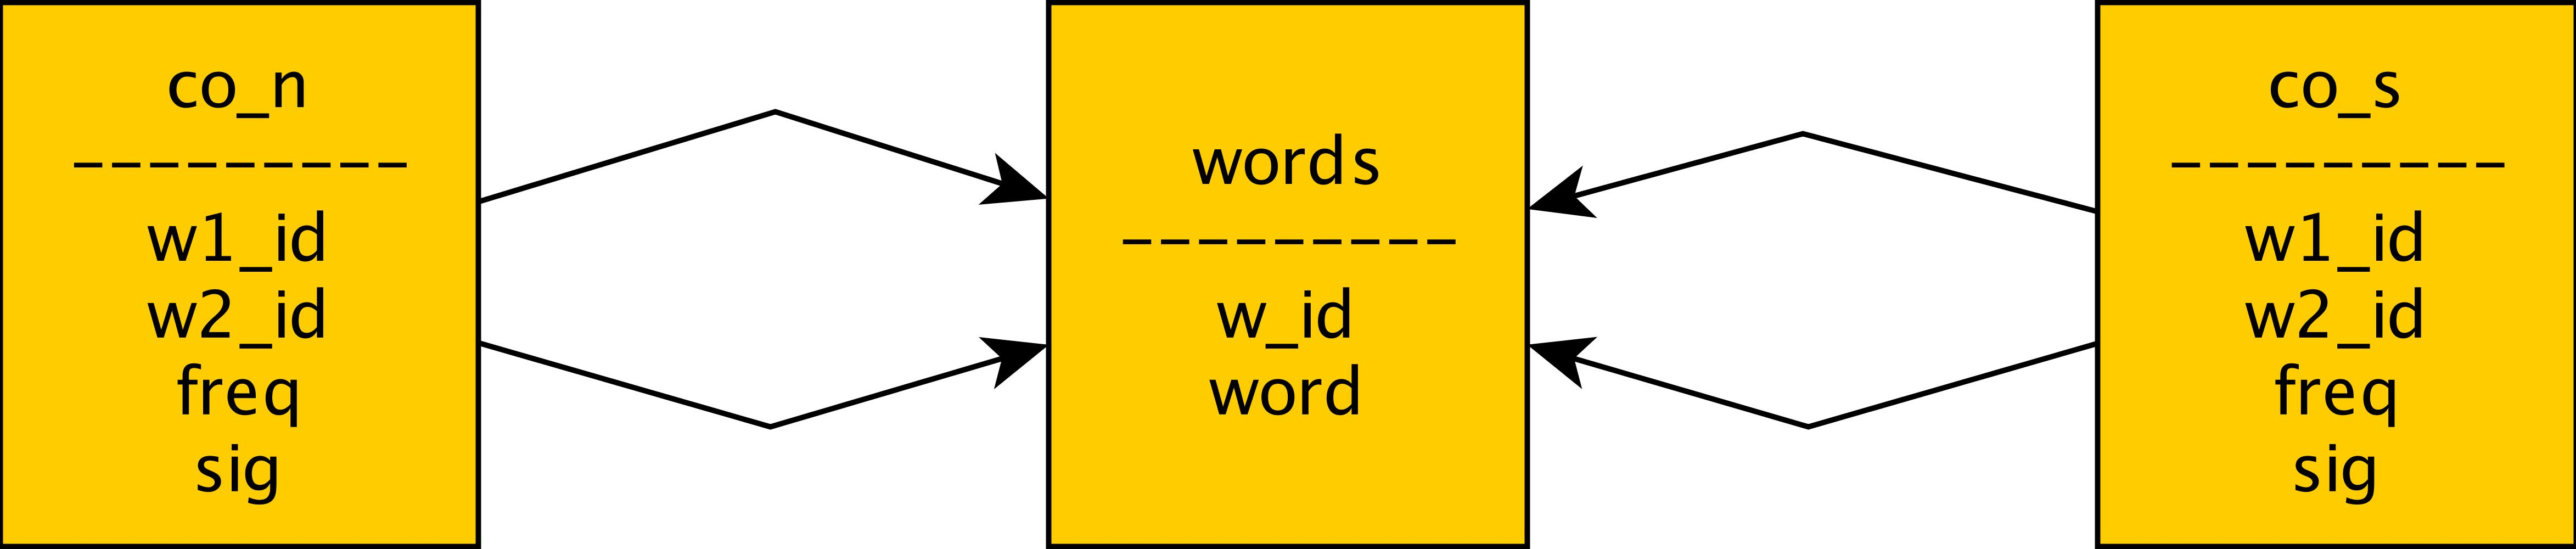
\includegraphics[scale=0.055]{images/mysql_schema}
\caption{MySQL Schema}
\label{fig:mysql_schema}
\end{minipage}
\hspace{0.5cm}
\begin{minipage}[b]{0.45\linewidth}
\centering
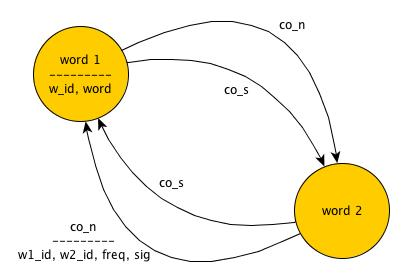
\includegraphics[scale=0.075]{images/graph_schema.jpg}
\caption{Graph}
\label{fig:graph_schema}
\end{minipage}
\end{figure}
\end{frame}

\begin{frame}\frametitle{Testdaten}
	\begin{table}
	\begin{tabular}{|l|r|r|r|}
		\hline
		Datenbank & Knoten & \multicolumn{2}{|c|}{Kanten}\\
		\hline
		 & words & co\_{}s & co\_{}n \\
		\hline
		\hline
		deu\_{}news\_{}2009\_{}10K & 39334 & 22062 & 5887\\
		\hline
		deu\_{}news\_{}2009\_{}100K & 191041 & 297422 & 69297\\
		\hline
		deu\_{}news\_{}2009\_{}300K & 390178 & 953218 & 196122\\
		\hline
		deu\_{}news\_{}2009\_{}1M & 830641 & 3349314 & 584402\\
		\hline
		deu\_{}news\_{}2009\_{}3M & 1623621 & 10596746 & 1546638\\
		\hline
		deu\_{}news\_{}2009\_{}10M & 3309332 & 37393614 & 4412321\\
		\hline
	\end{tabular}
	\caption{Kookkurrenzgraphen des Wortschatz Leipzig}
	\end{table}
\end{frame}

\begin{frame}\frametitle{Testabfragen}
\begin{description}
\item[Query 1]Finde alle Satz- oder Nachbarschaftskookkurrenzen eines Wortes. Gib Frequenz, Signifikanz und die beteiligten Wörter der Kookkurrenz aus.
\item[Query 2]Finde alle Satz- oder Nachbarschaftskookkurrenzen der Nachbarn eines Wortes. Gib Frequenz, Signifikanz und die beteiligten Wörter der Kookkurrenz aus.
\item[Query 3]Finde alle Satz- oder Nachbarschaftskookkurrenzen zwischen den Nachbarn eines Wortes. Gib Frequenz, Signifikanz und die beteiligten Wörter der Kookkurrenz aus.
\end{description}
\end{frame}

\section{Durchführung}
\begin{frame}\frametitle{Benchmark-Framework} 
	\begin{itemize}
		\item Verbindung zu MySQL und GraphDBs
		\item Importieren der Datenbasis aus MySQL in GraphDB
		\item Formulieren von DB-spezifischer Anfragen (Benchmark)
		\item Durchführen von Benchmarks und Messen der Ausführungszeit
		\item Export der Ergebnisse (csv)
		\item Konfiguration über Java Property Dateien
		\item Erweiterbarkeit
		\item Git-Repository unter \href{https://github.com/s1ck/IR15}{https://github.com/s1ck/IR15}

	\end{itemize} 
\end{frame}

\section{Auswertung}
\begin{frame}\frametitle{Gegenüberstellung}

\setbeamerfont{child}{size=\tiny}
\usebeamerfont{child}
	\renewcommand{\arraystretch}{1.5}
	
	\begin{table}[ht]
	\begin{tabular}{|l||p{2.5cm}|p{2.5cm}|p{2.5cm}|}
	\hline 
	 & \textbf{Neo4j} & \textbf{OrientDB} & \textbf{DEX} \\ 
	\hline
	Performance Import & $++$ & $--$ & ++ \\ 
	\hline 
	Performance Query 1 & ++ & ++* & ++ \\ 
	\hline 
	Performance Query 2 & ++ & +* & + \\ 
	\hline 
	Performance Query 3 & + & +* & ++ \\ 
	\hline
	Community & ++ & + & $--$ \\ 
	\hline 
	Dokumentation & ++ & ++ & $-$ \\
	\hline 
	Anfrage & Java API, Cypher, Gremlin & Java API, SQL, Gremlin & Java API \\
	\hline
	Implementiert in & Java & Java & C++ (Core), Java (API) \\
	\hline 
	Lizenz & GPL (Community Edition) & Apache License 2.0 & kommerziell	 \\ 
	\hline 
	\end{tabular}
	\caption{Gegenüberstellung der verwendeten Graphdatenbanken (* bis einschließlich deu\textunderscore news\textunderscore 300K)}
	\label{tab:compare}
	\end{table}
\normalfont
\end{frame}

\begin{frame}\frametitle{Teilergebnisse Beispiel}

\begin{figure}[ht]
\begin{minipage}[b]{0.45\linewidth}
\centering
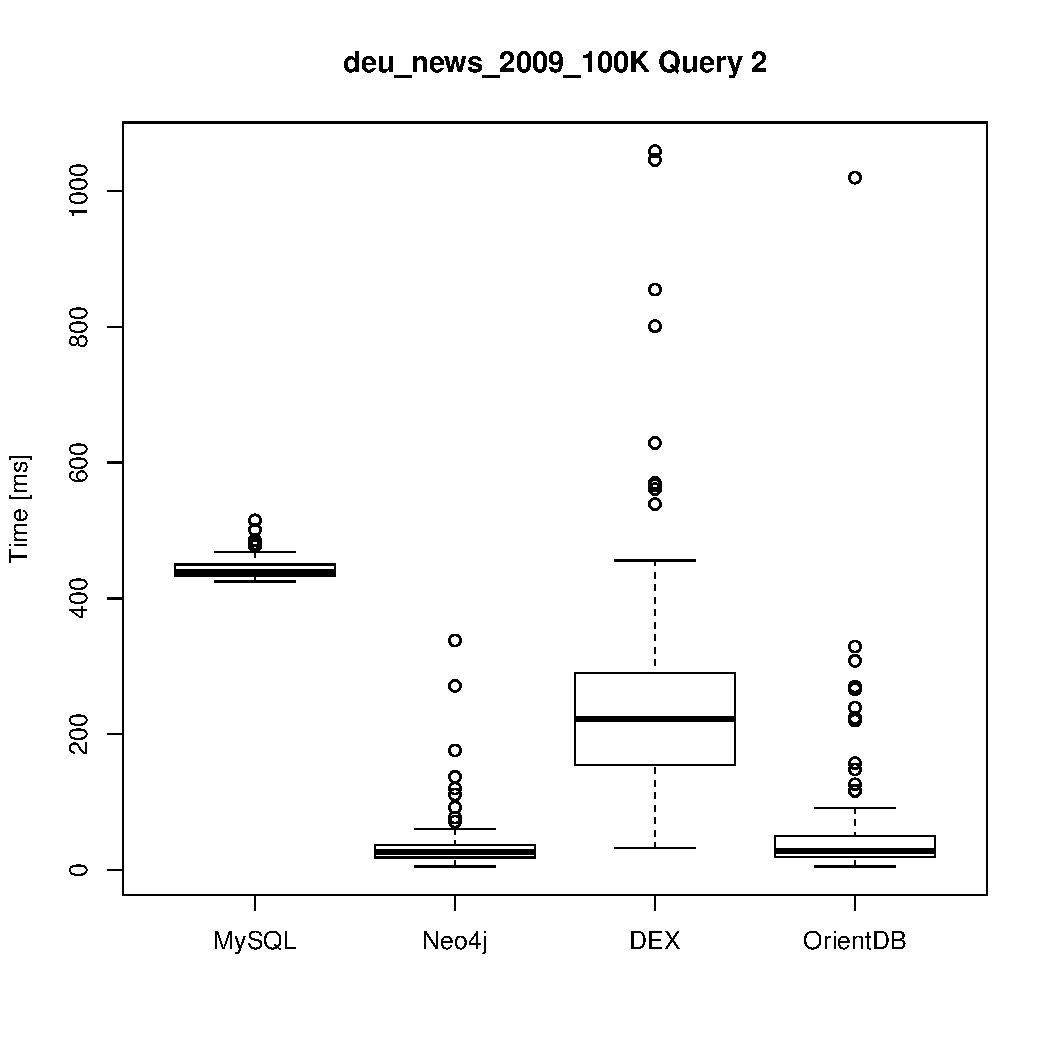
\includegraphics[scale=0.3]{../results/cold caches/images/100K_query2_boxplot.pdf}
\caption{Beispiel Boxplot}
\label{fig:mysql_schema}
\end{minipage}
\hspace{0.5cm}
\begin{minipage}[b]{0.45\linewidth}
\centering
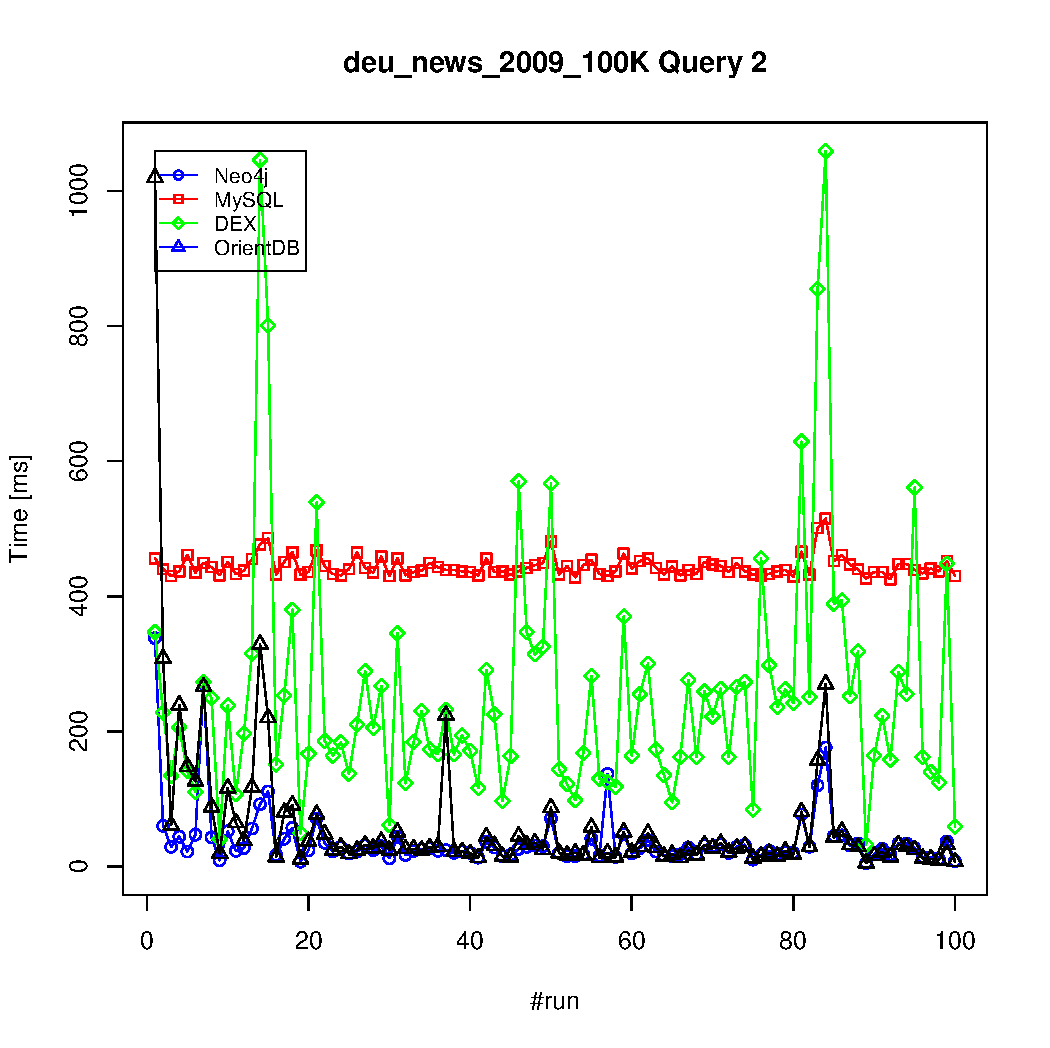
\includegraphics[scale=0.3]{../results/cold caches/images/100K_query2_perf.pdf}
\caption{Beispiel Performance}
\label{fig:graph_schema}
\end{minipage}
\end{figure}
\end{frame}

\begin{frame}\frametitle{Ergebnisse Query 2}
\begin{figure}[ht]
\centering
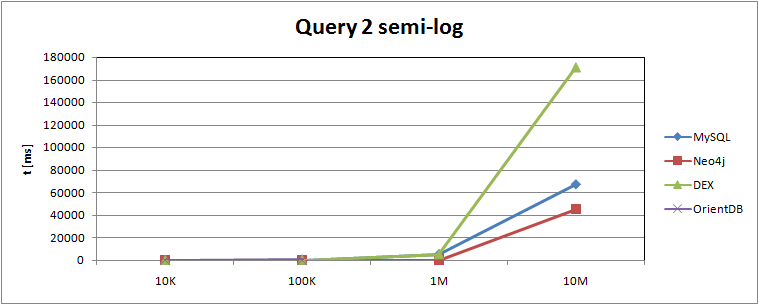
\includegraphics[scale=0.3]{../results/cold caches/images/query2_semi-log}
\label{fig:mysql_schema}
\end{figure}
\begin{figure}[ht]
\centering
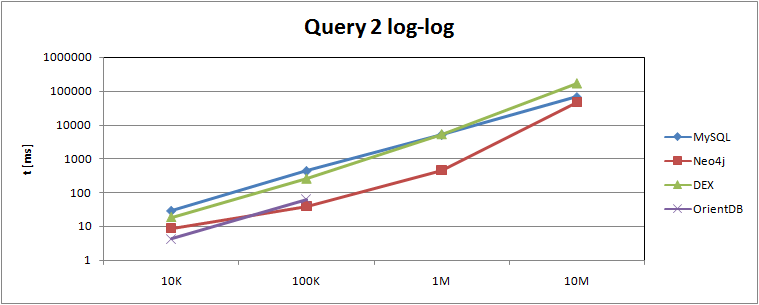
\includegraphics[scale=0.3]{../results/cold caches/images/query2_log-log}
\label{fig:mysql_schema}
\end{figure}
\end{frame}

\begin{frame}\frametitle{Ergebnisse Query 3}
\begin{figure}[ht]
\centering
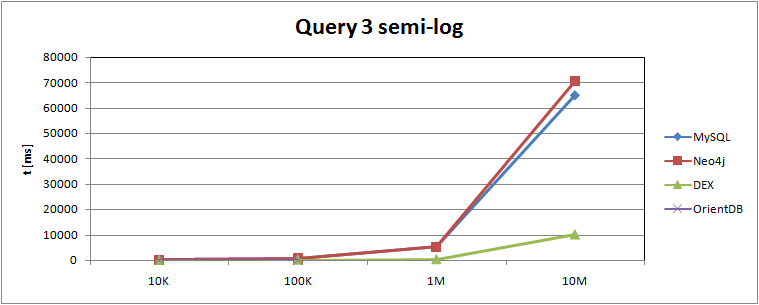
\includegraphics[scale=0.3]{../results/cold caches/images/query3_semi-log}
\label{fig:mysql_schema}
\end{figure}
\begin{figure}[ht]
\centering
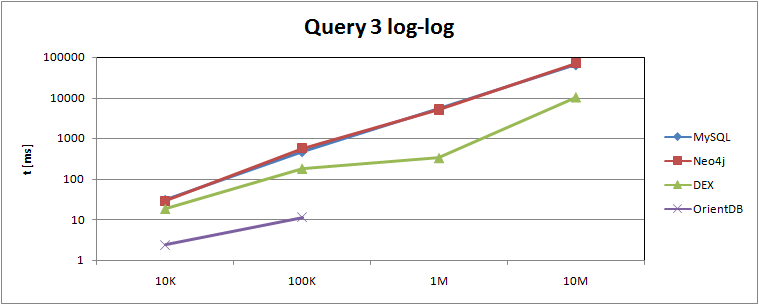
\includegraphics[scale=0.3]{../results/cold caches/images/query3_log-log}
\label{fig:mysql_schema}
\end{figure}
\end{frame}

\begin{frame}\frametitle{Problemverhalten von OrientDB}
\begin{figure}[ht]
\centering
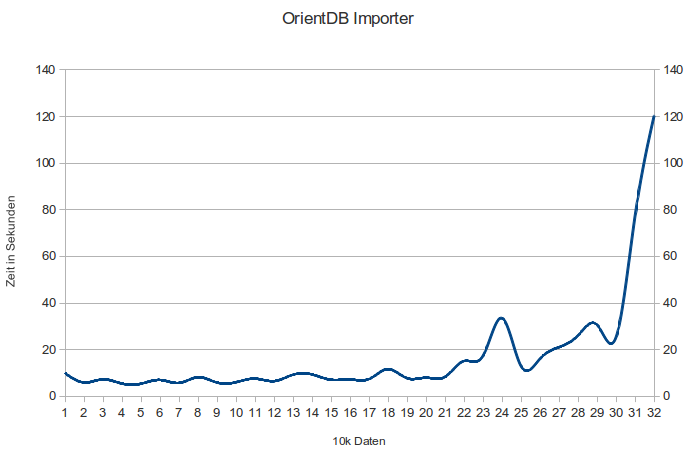
\includegraphics[scale=0.28]{../report/pics/OrientImporter}
\label{fig:mysql_schema}
\end{figure}
\end{frame}

\begin{frame}\frametitle{Empfehlung}
	\begin{itemize}
		\item Als GraphDB für den Anwendungsfall empfehlen wir Neo4j
		\item Gründe: Performanz, Dokumentation, aktive Community, Anfragesprache Cypher
		\item Weiterführende Evaluation im Zusammenhang mit Kookkurrenzgraphen und spezialisierten Anfragen (Pfadsuche, Matching) wird empfohlen
	\end{itemize} 
\end{frame}

\begin{frame}
	\begin{center}
		\begin{Huge}
			Ende
		\end{Huge}
	\end{center}
\end{frame}

\end{document}